\documentclass[../AnalysisNoteJBuxton.tex]{subfiles}
\begin{document}

\subsection{Residual Correlations}
\label{ResidualCorrelations}

The purpose of this analysis is study the interaction and scale of the emitting source of the pairs.
In order to obtain correct results, it is important for our particle collections to consist of primary particles.
In practice, this is difficult to achieve for our $\Lambda$ and $\bar{\Lambda}$ collections.
Many of our $\Lambda$ particles are not primary, but originate as decay products from other hyperons, including $\Sigma^{0}$, $\Xi^{0}$, $\Xi^{-}$ and $\Sigma^{*(+,-,0)}(1385)$.  Additionally, many of our K particles are not primary, but decay from K$^{*(+,-,0)}(892)$ parents.
In these decays, the $\Lambda$ carries away a momentum very similar to that of its parent.
As a result, the correlation function between a secondary $\Lambda$ and, for instance, a K$^{+}$  will be sensitive to, and dependent upon, the interaction between the parent of the $\Lambda$ and the K$^{+}$.
In effect, the correlation between the parent of the $\Lambda$ and the K$^{+}$ (ex. $\Sigma^{0}$K$^{+}$) will be visible, although smeared out, in the $\Lambda$K$^{+}$ data; we call this a residual correlation resulting from feed-down.
The contributions from the primary correlation, residual correlations, and fake pairs on the finally measure data is shown schematically in Figure \ref{fig:ResidualsCartoon}.
Residual correlations are important in an analysis when three criteria are met \cite{Kisiel:2014mma}: i) the parent correlation signal is large, ii) a large fraction of pairs in the sample originate from the particular parent system, and iii) the decay momenta are comparable to the expected correlation width in \textit{k}*. 


\begin{figure}[h]
  \centering
  \includegraphics[width=\textwidth]{5_Fitting/Figures/ResidualCartoons_p3.pdf}
  \caption[Residual Contributions Cartoon]{A schematic representation of the contributions to the finally measured data from the primary correlation, residual correlations, and fake pairs.}
  \label{fig:ResidualsCartoon}
\end{figure}



As it is difficult for us to eliminate these residual correlations in our analyses, we must attempt to account for them in our fitter.
To achieve this, we will simultaneously fit the data for both the primary correlation function and the residual correlations.  For example, in the simple case of a $\Lambda$K$^{+}$ analysis with residuals arising solely from $\Sigma^{0}$K$^{+}$ feed-down:

\begin{equation}
\begin{array}{l}
\vspace{4mm}
 C_{measured}(k^{*}_{\Lambda K^{+}}) = 1 + \lambda_{\Lambda K^{+}}[C_{\Lambda K^{+}}(k^{*}_{\Lambda K^{+}})-1] + \lambda_{\Sigma^{0}K^{+}}[C_{\Sigma^{0}K^{+}}(k^{*}_{\Lambda K^{+}})-1] \\
\vspace{2mm}
  ~~~~~C_{\Sigma^{0}K^{+}}(k^{*}_{\Lambda K^{+}}) \equiv \frac{\sum\limits_{k^{*}_{\Sigma^{0}K^{+}}} C_{\Sigma^{0}K^{+}}\left(k^{*}_{\Sigma^{0}K^{+}}\right) T\left(k^{*}_{\Sigma^{0}K^{+}},k^{*}_{\Lambda K^{+}}\right)}{\sum\limits_{k^{*}_{\Sigma^{0}K^{+}}} T\left(k^{*}_{\Sigma^{0}K^{+}},k^{*}_{\Lambda K^{+}}\right)}
\end{array} 
\label{eqn:SimpleResiduals}
\end{equation}

$C_{\Sigma^{0}K^{+}}(k^{*}_{\Sigma^{0}K^{+}})$ is the $\Sigma^{0}$K$^{+}$ correlation function from, for instance, Equation \ref{eqn:LednickyEqn}, and $T$ is the transform matrix generated with THERMINATOR.  The transform matrix is formed for a given parent pair, AB, by taking all $\Lambda$K pairs originating from AB, calculating the relative momentum of the parents (\textit{k}*$_{AB}$) and daughters (\textit{k}*$_{\Lambda K}$), and filling a two-dimensional histogram with the values. The transform matrix is essentially an unnormalized probability distribution mapping the \textit{k}* of the parent pair to that of the daughter pair when one or both parents decay.  An example of such transform matrices can be found in Figures \ref{fig:TransformMatricesLamKchP} and \ref{fig:TransformMatricesALamKchP}.

  The above equation can be easily extended to include feed-down from more sources:

\begin{equation}
\begin{array}{l}
\vspace{4mm}
\begin{split}
 C_{measured}(k^{*}_{\Lambda K}) & = 1 + \lambda_{\Lambda K}[C_{\Lambda K}(k^{*}_{\Lambda K})-1] + \lambda_{\Sigma^{0}K}[C_{\Sigma^{0}K}(k^{*}_{\Lambda K})-1] + ... \\ &
 + \lambda_{P_{1}P_{2}}[C_{P_{1}P_{2}}(k^{*}_{\Lambda K})-1] + \lambda_{other}[C_{other}(k^{*}_{\Lambda K})-1] 
\end{split}
\\
\vspace{2mm}
  ~~~~~C_{P_{1}P_{2}}(k^{*}_{\Lambda K}) \equiv \frac{\sum\limits_{k^{*}_{P_{1}P_{2}}} C_{P_{1}P_{2}}\left(k^{*}_{P_{1}P_{2}}\right) T\left(k^{*}_{P_{1}P_{2}},k^{*}_{\Lambda K}\right)}{\sum\limits_{k^{*}_{P_{1}P_{2}}} T\left(k^{*}_{P_{1}P_{2}},k^{*}_{\Lambda K}\right)}
\end{array} 
\label{eqn:ResidualsFull}
\end{equation}

  Or, more compactly:

\begin{equation}
 C_{measured}(k^{*}_{\Lambda K}) = 1 + \sum\limits_{i}  \lambda_{i}[C_{i}(k^{*}_{\Lambda K})-1]
\label{eqn:Residuals}
\end{equation}



\begin{figure}[h!]
  \centering
  %%----start of first subfigure---  
  \subfloat[Transform matrix for $\Sigma$K$^{+}$ pairs into $\Lambda$K$^{+}$]{
    \label{fig:TransformMatricesLamKchP:a}
    \includegraphics[width=0.49\textwidth]{5_Fitting/Figures/fSigToLamKchPTransform.pdf}}%\\
  %%----start of second subfigure---
  \subfloat[Transform matrix for $\Xi^{-}$K$^{+}$ pairs into $\Lambda$K$^{+}$]{
    \label{fig:TransformMatricesLamKchP:b}
    \includegraphics[width=0.49\textwidth]{5_Fitting/Figures/fXiCToLamKchPTransform.pdf}} \\
  %%----start of third subfigure---
  \subfloat[Transform matrix for $\Xi^{0}$K$^{+}$ pairs into $\Lambda$K$^{+}$]{
    \label{fig:TransformMatricesLamKchP:c}
    \includegraphics[width=0.49\textwidth]{5_Fitting/Figures/fXi0ToLamKchPTransform.pdf}}
  %%----start of fourth subfigure---
  \subfloat[Transform matrix for $\Omega^{-}$K$^{+}$ pairs into $\Lambda$K$^{+}$]{
    \label{fig:TransformMatricesLamKchP:d}
    \includegraphics[width=0.49\textwidth]{5_Fitting/Figures/fOmegaToLamKchPTransform.pdf}} \\                   
  %%----overall caption----
  \caption[Transform Matrices for $\Lambda$K$^{+}$ Analysis]{Transform Matrices generated with THERMINATOR for $\Lambda$K$^{+}$ Analysis}
  \label{fig:TransformMatricesLamKchP}
\end{figure}


\begin{figure}[h!]
  \centering
  %%----start of first subfigure---
  \subfloat[Transform matrix for $\bar{\Sigma}$K$^{+}$ pairs into $\bar{\Lambda}$K$^{+}$]{
    \label{fig:TransformMatricesALamKchP:a}
    \includegraphics[width=0.49\textwidth]{5_Fitting/Figures/fASigToALamKchPTransform.pdf}}
  %%----start of second subfigure---
  \subfloat[Transform matrix for $\bar{\Xi}^{+}$K$^{+}$ pairs into $\bar{\Lambda}$K$^{+}$]{
    \label{fig:TransformMatricesALamKchP:b}
    \includegraphics[width=0.49\textwidth]{5_Fitting/Figures/fAXiCToALamKchPTransform.pdf}} \\
  %%----start of third subfigure---
  \subfloat[Transform matrix for $\bar{\Xi}^{0}$K$^{+}$ pairs into $\bar{\Lambda}$K$^{+}$]{
    \label{fig:TransformMatricesALamKchP:c}
    \includegraphics[width=0.49\textwidth]{5_Fitting/Figures/fAXi0ToALamKchPTransform.pdf}}
  %%----start of fourth subfigure---
  \subfloat[Transform matrix for $\bar{\Omega}^{+}$K$^{+}$ pairs into $\bar{\Lambda}$K$^{+}$]{
    \label{fig:TransformMatricesALamKchP:d}
    \includegraphics[width=0.49\textwidth]{5_Fitting/Figures/fAOmegaToALamKchPTransform.pdf}}                    
  %%----overall caption----
  \caption[Transform Matrices for $\bar{\Lambda}$K$^{+}$ Analysis]{Transform Matrices generated with THERMINATOR for $\bar{\Lambda}$K$^{+}$ Analysis}
  \label{fig:TransformMatricesALamKchP}
\end{figure}


So, in practice, we model the correlation function of the parents, and run the correlation function through the appropriate transform matrix to determine the contribution to the daughter correlation function.  A few questions still remain.  First, what $\lambda$ values should be used in the above equation?  One option would be to leave all of these $\lambda$-parameters free during the fit process.  However, this would introduce a huge number of new parameters into the fitter, and would make the fit results less trustworthy.  The $\lambda$ parameters roughly dictate the strength of the parent contribution to the daughter pair.  Additionally, as found in \cite{Salzwedel:2241303}, the reconstruction efficiency for primary $\Lambda$ particles is nearly equal to that of $\Lambda$ particles originating from $\Sigma$, $\Sigma^{*}$, $\Xi^{0}$, $\Xi^{-}$, and $\Omega$ hyperons.  Therefore, the $\lambda$ parameter for parent system AB can be estimated using THERMINATOR as the total number of $\Lambda$K pairs originating from AB (N$_{AB}$) divided by the total number of $\Lambda$K pairs (N$_{Total}$):

\begin{equation}
\lambda_{AB} = \frac{N_{AB}}{N_{Total}}
\end{equation}


%\clearpage
\begin{table}[htbp]
 \centering
 \renewcommand{\arraystretch}{1.2}
 %------------------------------------LamKchP
 \begin{minipage}{0.3\textwidth}
  \centering
  \begin{tabular}{|c|c|}
   \multicolumn{2}{c}{$\Lambda$K$^{+}$ Residuals} \\
   \hline
   \textbf{Pair System} & \textbf{$\lambda$ value} \\
   \hlineB{3.0}
   \multicolumn{2}{|c|}{3 Residuals} \\
   \hlineB{3.0}   
   $\Lambda$K$^{+}$ & 0.154 \\
   $\Sigma^{0}$K$^{+}$ & 0.099 \\
   $\Xi^{0}$K$^{+}$ & 0.072 \\
   $\Xi^{-}$K$^{+}$ & 0.069 \\
   Other & 0.558 \\
   Fakes & 0.048 \\
   \hlineB{3.0}
   \multicolumn{2}{|c|}{10 Residuals} \\
   \hlineB{3.0}
   $\Lambda$K$^{+}$ & 0.154 \\
   $\Sigma^{0}$K$^{+}$ & 0.099 \\
   $\Xi^{0}$K$^{+}$ & 0.072 \\
   $\Xi^{-}$K$^{+}$ & 0.069 \\
   $\Sigma^{*+}$K$^{+}$ & 0.046 \\
   $\Sigma^{*-}$K$^{+}$ & 0.042 \\
   $\Sigma^{*0}$K$^{+}$ & 0.042 \\
   $\Lambda$K$^{*0}$ & 0.039 \\
   $\Sigma^{0}$K$^{*0}$ & 0.035 \\
   $\Xi^{0}$K$^{*0}$ & 0.025 \\
   $\Xi^{-}$K$^{*0}$ & 0.024 \\
   Other & 0.305 \\
   Fakes & 0.048 \\  
   \hline 
  \end{tabular}
 \end{minipage}
 %------------------------------------ALamKchM
 \begin{minipage}{0.3\textwidth}
  \centering
  \begin{tabular}{|c|c|}
   \multicolumn{2}{c}{$\bar{\Lambda}$K$^{-}$ Residuals} \\
   \hline
   \textbf{Pair System} & \textbf{$\lambda$ value} \\
   \hlineB{3.0}
   \multicolumn{2}{|c|}{3 Residuals} \\
   \hlineB{3.0}   
   $\bar{\Lambda}$K$^{-}$ & 0.158 \\
   $\bar{\Sigma}^{0}$K$^{-}$ & 0.102 \\
   $\bar{\Xi}^{0}$K$^{-}$ & 0.067 \\
   $\bar{\Xi}^{+}$K$^{-}$ & 0.065 \\
   Other & 0.560 \\
   Fakes & 0.048 \\
   \hlineB{3.0}
   \multicolumn{2}{|c|}{10 Residuals} \\
   \hlineB{3.0}
   $\bar{\Lambda}$K$^{-}$ & 0.158 \\
   $\bar{\Sigma}^{0}$K$^{-}$ & 0.102 \\
   $\bar{\Xi}^{0}$K$^{-}$ & 0.067 \\
   $\bar{\Xi}^{+}$K$^{-}$ & 0.065 \\
   $\bar{\Sigma}^{*-}$K$^{-}$ & 0.046 \\
   $\bar{\Sigma}^{*+}$K$^{-}$ & 0.045 \\
   $\bar{\Sigma}^{*0}$K$^{-}$ & 0.040 \\
   $\bar{\Lambda}\bar{\mathrm{K}}^{*0}$ & 0.041 \\
   $\bar{\Sigma}^{0}\bar{\mathrm{K}}^{*0}$ & 0.036 \\
   $\bar{\Xi}^{0}\bar{\mathrm{K}}^{*0}$ & 0.024 \\
   $\bar{\Xi}^{+}\bar{\mathrm{K}}^{*0}$ & 0.023 \\
   Other & 0.305 \\
   Fakes & 0.048 \\
   \hline      
  \end{tabular}
 \end{minipage}  
 \caption{$\lambda$ values for the individual components of the $\Lambda$K$^{+}$ (left) and $\bar{\Lambda}$K$^{-}$ (right) correlation functions for the case of 3 and 10 residual contributions.}
 \label{tab:LambdaValues_LamKchP}
\end{table}




%\clearpage
\begin{table}[htbp]
 \centering
 \renewcommand{\arraystretch}{1.2}
  %------------------------------------LamKchM
 \begin{minipage}{0.3\textwidth}
  \centering
  \begin{tabular}{|c|c|}
   \multicolumn{2}{c}{$\Lambda$K$^{-}$ Residuals} \\
   \hline
   \textbf{Pair System} & \textbf{$\lambda$ value} \\
   \hlineB{3.0}
   \multicolumn{2}{|c|}{3 Residuals} \\
   \hlineB{3.0}   
   $\Lambda$K$^{-}$ & 0.154 \\
   $\Sigma^{0}$K$^{-}$ & 0.099 \\
   $\Xi^{0}$K$^{-}$ & 0.071 \\
   $\Xi^{-}$K$^{-}$ & 0.068 \\
   Other & 0.561 \\
   Fakes & 0.048 \\
   \hlineB{3.0}
   \multicolumn{2}{|c|}{10 Residuals}\\
   \hlineB{3.0}
   $\Lambda$K$^{-}$ & 0.154 \\
   $\Sigma^{0}$K$^{-}$ & 0.099 \\
   $\Xi^{0}$K$^{-}$ & 0.071 \\
   $\Xi^{-}$K$^{-}$ & 0.068 \\
   $\Sigma^{*+}$K$^{-}$ & 0.046 \\
   $\Sigma^{*-}$K$^{-}$ & 0.041 \\
   $\Sigma^{*0}$K$^{-}$ & 0.041 \\
   $\Lambda\bar{\mathrm{K}}^{*0}$ & 0.039 \\
   $\Sigma^{0}\bar{\mathrm{K}}^{*0}$ & 0.035 \\
   $\Xi^{0}\bar{\mathrm{K}}^{*0}$ & 0.025 \\
   $\Xi^{-}\bar{\mathrm{K}}^{*0}$ & 0.024 \\
   Other & 0.308 \\
   Fakes & 0.048 \\
   \hline   
  \end{tabular}
 \end{minipage}
 %------------------------------------ALamKchP
 \begin{minipage}{0.3\textwidth}
  \centering
  \begin{tabular}{|c|c|}
   \multicolumn{2}{c}{$\bar{\Lambda}$K$^{+}$ Residuals} \\
   \hline
   \textbf{Pair System} & \textbf{$\lambda$ value} \\
   \hlineB{3.0}
   \multicolumn{2}{|c|}{3 Residuals} \\
   \hlineB{3.0}   
   $\bar{\Lambda}$K$^{+}$ & 0.158 \\
   $\bar{\Sigma}^{0}$K$^{+}$ & 0.103 \\
   $\bar{\Xi}^{0}$K$^{+}$ & 0.068 \\
   $\bar{\Xi}^{+}$K$^{+}$ & 0.066 \\
   Other & 0.557 \\
   Fakes & 0.048 \\
   \hlineB{3.0}
   \multicolumn{2}{|c|}{10 Residuals} \\
   \hlineB{3.0}
   $\bar{\Lambda}$K$^{+}$ & 0.158 \\
   $\bar{\Sigma}^{0}$K$^{+}$ & 0.103 \\
   $\bar{\Xi}^{0}$K$^{+}$ & 0.068 \\
   $\bar{\Xi}^{+}$K$^{+}$ & 0.066 \\
   $\bar{\Sigma}^{*-}$K$^{+}$ & 0.046 \\
   $\bar{\Sigma}^{*+}$K$^{+}$ & 0.045 \\
   $\bar{\Sigma}^{*0}$K$^{+}$ & 0.041 \\
   $\bar{\Lambda}$K$^{*0}$ & 0.041 \\
   $\bar{\Sigma}^{0}$K$^{*0}$ & 0.036 \\
   $\bar{\Xi}^{0}$K$^{*0}$ & 0.024 \\
   $\bar{\Xi}^{+}$K$^{*0}$ & 0.023 \\
   Other & 0.301 \\
   Fakes & 0.048 \\
   \hline   
  \end{tabular}
 \end{minipage} 
 \caption{$\lambda$ values for the individual components of the $\Lambda$K$^{-}$ (left) and $\bar{\Lambda}$K$^{+}$ (right) correlation functions for the case of 3 and 10 residual contributions.}
 \label{tab:LambdaValues_LamKchM}
\end{table}


%\clearpage
\begin{table}[htbp]
 \centering
  \renewcommand{\arraystretch}{1.2}
  %------------------------------------LamK0
 \begin{minipage}{0.3\textwidth}
  \centering
  \begin{tabular}{|c|c|}
   \multicolumn{2}{c}{$\Lambda$K$^{0}_{\mathrm{S}}$ Residuals} \\
   \hline
   \textbf{Pair System} & \textbf{$\lambda$ value} \\
   \hlineB{3.0}
   \multicolumn{2}{|c|}{3 Residuals} \\
   \hlineB{3.0}   
   $\Lambda$K$^{0}_{\mathrm{S}}$ & 0.165 \\
   $\Sigma^{0}$K$^{0}_{\mathrm{S}}$ & 0.107 \\
   $\Xi^{0}$K$^{0}_{\mathrm{S}}$ & 0.077 \\
   $\Xi^{-}$K$^{0}_{\mathrm{S}}$ & 0.075 \\
   Other & 0.528 \\
   Fakes & 0.048 \\
   \hlineB{3.0}
   \multicolumn{2}{|c|}{10 Residuals} \\
   \hlineB{3.0}   
   $\Lambda$K$^{0}_{\mathrm{S}}$ & 0.165 \\
   $\Sigma^{0}$K$^{0}_{\mathrm{S}}$ & 0.107 \\
   $\Xi^{0}$K$^{0}_{\mathrm{S}}$ & 0.077 \\
   $\Xi^{-}$K$^{0}_{\mathrm{S}}$ & 0.075 \\
   $\Sigma^{*+}$K$^{0}_{\mathrm{S}}$ & 0.050 \\
   $\Sigma^{*-}$K$^{0}_{\mathrm{S}}$ & 0.045 \\
   $\Sigma^{*0}$K$^{0}_{\mathrm{S}}$ & 0.045 \\
   $\Lambda$K$^{*0}$ & 0.019 \\
   $\Sigma^{0}$K$^{*0}$ & 0.017 \\
   $\Xi^{0}$K$^{*0}$ & 0.012 \\
   $\Xi^{-}$K$^{*0}$ & 0.012 \\
   Other & 0.329 \\
   Fakes & 0.048 \\
   \hline   
  \end{tabular}
 \end{minipage}
 %------------------------------------ALamK0
 \begin{minipage}{0.3\textwidth}
  \centering
  \begin{tabular}{|c|c|}
   \multicolumn{2}{c}{$\bar{\Lambda}$K$^{0}_{\mathrm{S}}$ Residuals} \\
   \hline
   \textbf{Pair System} & \textbf{$\lambda$ value} \\
   \hlineB{3.0}
   \multicolumn{2}{|c|}{3 Residuals} \\
   \hlineB{3.0}   
   $\bar{\Lambda}$K$^{0}_{\mathrm{S}}$ & 0.169 \\
   $\bar{\Sigma}^{0}$K$^{0}_{\mathrm{S}}$ & 0.111 \\
   $\bar{\Xi}^{0}$K$^{0}_{\mathrm{S}}$ & 0.073 \\
   $\bar{\Xi}^{+}$K$^{0}_{\mathrm{S}}$ & 0.071 \\
   Other & 0.528 \\
   Fakes & 0.048 \\
   \hlineB{3.0}
   \multicolumn{2}{|c|}{10 Residuals} \\
   \hlineB{3.0}   
   $\bar{\Lambda}$K$^{0}_{\mathrm{S}}$ & 0.169 \\
   $\bar{\Sigma}^{0}$K$^{0}_{\mathrm{S}}$ & 0.111 \\
   $\bar{\Xi}^{0}$K$^{0}_{\mathrm{S}}$ & 0.073 \\
   $\bar{\Xi}^{+}$K$^{0}_{\mathrm{S}}$ & 0.071 \\
   $\bar{\Sigma}^{*-}$K$^{0}_{\mathrm{S}}$ & 0.050 \\
   $\bar{\Sigma}^{*+}$K$^{0}_{\mathrm{S}}$ & 0.049 \\
   $\bar{\Sigma}^{*0}$K$^{0}_{\mathrm{S}}$ & 0.044 \\
   $\bar{\Lambda}$K$^{*0}$ & 0.020 \\
   $\bar{\Sigma}^{0}$K$^{*0}$ & 0.017 \\
   $\bar{\Xi}^{0}$K$^{*0}$ & 0.011 \\
   $\bar{\Xi}^{+}$K$^{*0}$ & 0.011 \\
   Other & 0.326 \\
   Fakes & 0.048 \\
   \hline   
  \end{tabular}
 \end{minipage} 
 \caption{$\lambda$ values for the individual components of the $\Lambda$K$^{0}_{\mathrm{S}}$ (left) and $\bar{\Lambda}$K$^{0}_{\mathrm{S}}$ (right) correlation functions for the case of 3 and 10 residual contributions.}
 \label{tab:LambdaValues_LamK0}
\end{table}


Now, the remaining question is how do we model the parent correlation functions?  In an ideal world, we would simply look up the parent interaction in some table, and input this into our Lednicky equation (for the case of one or more charge neutral particle in the pair), or run it through the CoulombFitter machinery described in Sec. \ref{ModelCascadeKaon}.  Unfortunately, the world in which we live is not perfect, such a table does not exists, and little is know about the interaction between the residual pairs in this study.  One solution would be to introduce a set of scattering parameters and radii for each residual system.  However, as will the case of the $\lambda$-parameters above, this would introduce a large number of additional fit parameters, and would make our fitter too unconstrained and would yield untrustworthy results.  The second option, which is adopted in this analysis, is to assume all residual pairs have the same source size as the daughter pair, and all Coulomb-neutral residual pairs also share the same scattering parameters as the daughter pair (the case of charged pairs will be described below).

Concerning the radii of the residual parent pairs, it was suggested that these should be set to smaller values.  In the interest of minimizing the number of parameters in the fitter, we tested this by introducing an \textit{m}$_{\mathrm{T}}$-scaling of the parent radii.  The motivation for this scaling comes from the approximate \textit{m}$_{\mathrm{T}}$-scaling of the radii observed in \ref{fig:mTScalingOfRadii}.  To achieve this scaling, we assume the radii follow an inverse-square-root distribution: $R_{AB} = \alpha m_{\mathrm{T}}^{-1/2}$.  Then, it follows that we should scale the parent radii as:

\begin{equation}
R_{AB} = R_{\Lambda K}\left(\frac{m_{\mathrm{T},AB}}{m_{\mathrm{T},\Lambda K}}\right)^{-1/2}
\end{equation}

The values for $m_{\mathrm{T}}$ for each pair system was taken from THERMINATOR.  As the fitter dances around parameter space and selects new radii for the $\Lambda$K pairs, the radii of the residuals is scaled by the above factor.  In the end, this scaling factor made no significant difference in our fit results, so this complication is excluded from our final results.  Note that this is not surprising, as the most extreme scaling factor was, in the case of using 10 residual systems, between $\Lambda$K+ with $m_{\mathrm{T},\Lambda K+} \approx$ 1.4 GeV/$c^{2}$ and $\Xi^{-}$K$^{*0}$ with $m_{\mathrm{T},\Xi^{-} K^{*0}} \approx$ 1.8 GeV/$c^{2}$, resulting in a scale factor of $\approx$ 0.9.

Now, as hinted above, accounting for charged residuals adds a complication in that they necessitate the inclusion of the CoulombFitter into the process.  The complication of combining the two fitters is not troubling, but it increases the fitting time drastically (the parallelization of the CoulombFitter across a large number of GPU cores, to drastically decrease run-time, is currently underway).  We have two solutions to bypass such a large increase in run time.  First, we can use our experimental $\Xi^{\mathrm{ch}}$K$^{\mathrm{ch}}$ data to represent all charged parent pair system.  In this case, there is no need to make any assumption about scattering parameters or source sizes, as we already have the experimental data.  The downside is that, especially in the 30-50\% centrality bin, the error bars on the data are large.  Alternatively, we can assume the strong interaction is negligible in the charged residual, and generate the parent correlation function given radius and $\lambda$ parameters.  We find in our $\Xi^{\mathrm{ch}}$K$^{\mathrm{ch}}$ study that a Coulomb-only description of the system describes, reasonably well, the broad features of the correlation.  The strong interaction is necessary for the fine details.  However, as these correlations are run through a transform matrix, which largely flattens out and fine details, a Coulomb-only description should be sufficient.  In practice, this Coulomb-only scenario is achieved by first building a large number of Coulomb-only correlations for various radii and $\lambda$ parameter values, and interpolating from this grid during the fitting process.  We find consistent results between using the $\Xi$K data and the Coulomb-only interpolation method.  When the number of residual pairs used is increased to 10, so that pairs such as $\Sigma^{*+}$K$^{-}$ enter the picture, the Coulomb-only interpolation method is used.  In other words, the $\Xi$K experimental data is only used to model the $\Xi$K residual contribution, all other charged pairs are treated with the Coulomb-only interpolation method.

Two examples of how very different transform matrices can alter a correlation function are shown in Figures \ref{fig:Sig0KchPtoLamKchPTransform} and \ref{fig:LamKSt0toLamKchPTransform} below.  These figures were taken using parameter values obtained from fits to the data.  In the top left corner of the figures, the input correlation function (closed symbols) is shown together with the output, transformed, correlation function (open symbols).  In the bottom left, the transformed correlation is shown by itself.  This is especially helpful when the $\lambda$ parameter is very small, in which case the contribution in the top left can look flat, but the zoomed in view in the bottom left shows the structure.  The right two plots in each figure show the transform matrix without (top right) and with (bottom right) a log-scale on the z-axis.  Note, more examples of these transforms can be found in Sec. \ref{AdditionalFigures}.

\begin{figure}[h]
  \centering
  \includegraphics[width=\textwidth]{5_Fitting/Figures/Residuals_LamKchP_0010_Sig0KchP_MomResCrctn_NonFlatBgdCrctn_10Res_PrimMaxDecay4fm_UsingXiDataAndCoulombOnly.pdf}
  \caption[$\Sigma^{0}$K$^{+}$ Transform]{$\Sigma^{0}$K$^{+}$ Transform.  These figures were taken using parameter values obtained from fits to the data.  In the top left corner of the figures, the input correlation function (closed symbols) is shown together with the output, transformed, correlation function (open symbols).  In the bottom left, the transformed correlation is shown by itself.  The right two plots in each figure show the transform matrix without (top right) and with (bottom right) a log-scale on the z-axis.}
  \label{fig:Sig0KchPtoLamKchPTransform}
\end{figure}


\begin{figure}[h]
  \centering
  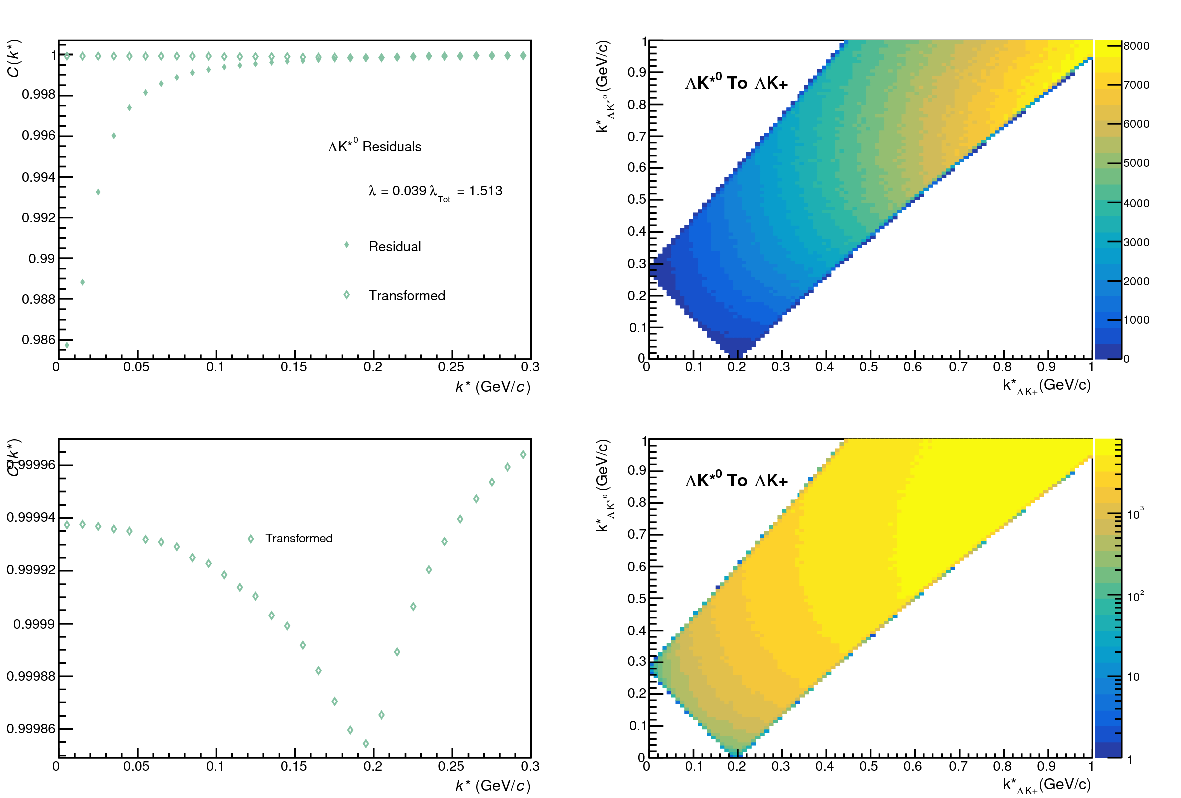
\includegraphics[width=\textwidth]{5_Fitting/Figures/Residuals_LamKchP_0010_LamKSt0_MomResCrctn_NonFlatBgdCrctn_10Res_PrimMaxDecay4fm_UsingXiDataAndCoulombOnly.pdf}
  \caption[$\Sigma^{0}$K$^{+}$ Transform]{$\Sigma^{0}$K$^{+}$ Transform.  These figures were taken using parameter values obtained from fits to the data.  In the top left corner of the figures, the input correlation function (closed symbols) is shown together with the output, transformed, correlation function (open symbols).  In the bottom left, the transformed correlation is shown by itself.  The right two plots in each figure show the transform matrix without (top right) and with (bottom right) a log-scale on the z-axis.}
  \label{fig:LamKSt0toLamKchPTransform}
\end{figure}

\clearpage

\end{document}